\section{The rewriter-prompt ladder and the style probe, in detail}
\label{app:mechanism}


\begin{table}[htbp]
\centering
\caption{The rewriter-prompt ladder. Rows run from the prompt farthest from the benchmark's (D4) to the benchmark's own (D1), with the untrained base and the verified arm above for reference; columns are R@1 on the easy tier, the hard tier and cross-language duplicates, mean $\pm$ sd over the same three seeds ($42$--$44$). The hard-tier column falls step by step from D1 to D4, the registered prediction that passed; the easy-tier column does not, since D2 and D3 outscore D1 and only D4 drops; on duplicates D4 tops every model including the base. Three notes: D1 is the recipe arm read at three seeds, so its numbers differ slightly from the eight-seed ones of Table~\ref{tab:controlled} ($62.38 \pm 0.85$ / $9.42 \pm 0.61$); D3 trained on the $5{,}591$ positives its prompt yielded rather than the matched $6{,}145$, which a control shows \emph{flatters} it on the hard tier; D4 attaches no negatives by design, and Table~\ref{tab:factorial} separates that from its prompt. On real duplicates only the contrasts between D4 and the rest replicate across seeds. The points are plotted in Figure~\ref{fig:inversion}.}
\label{tab:dose-full}
\small
\setlength{\tabcolsep}{4pt}
\begin{tabular}{@{}p{5.8cm}>{\centering\arraybackslash}p{2.3cm}>{\centering\arraybackslash}p{2.3cm}>{\centering\arraybackslash}p{2.6cm}@{}}
\toprule
Training set & Easy R@1 & Hard R@1 & Cross-language dup.\ R@1 \\
\midrule
Base 0.6B (untrained) & 8.32 & 0.00 & 84.73 \\
Verified arm & 17.05 $\pm$ 0.79 & 0.16 $\pm$ 0.06 & 56.52 $\pm$ 4.05 \\
D4: restatement prompt unrelated to the recipe & 30.03 $\pm$ 1.45 & 0.04 $\pm$ 0.02 & \textbf{93.81 $\pm$ 0.39} \\
D3: rewrite prompt in a different style & 67.88 $\pm$ 0.76 & 4.67 $\pm$ 0.40 & 65.39 $\pm$ 1.83 \\
D2: paraphrase of the benchmark's prompt & 67.54 $\pm$ 1.95 & 6.76 $\pm$ 1.01 & 68.02 $\pm$ 3.51 \\
D1: the benchmark's prompt ($=$ recipe arm) & 61.86 $\pm$ 0.52 & \textbf{9.90 $\pm$ 0.74} & 66.41 $\pm$ 1.78 \\
\bottomrule
\end{tabular}
\end{table}


\paragraph{The registered decay prediction, and its falsifier.}
The primary registration predicted that hard-tier R@1 would fall monotonically as the prompt moves away from the benchmark's, with a single falsifier at the far end: D4 scoring ${\ge}\,4.69$, half the $9.37$-point gain D1 had shown at seed $42$ when the prediction was written, would refute it. It was written after D1 and the controlled arms were measured and before D2--D4 existed. One weakness to admit: because its only falsifier sits at the D4 endpoint, the prediction would also have counted as passing had only the endpoints differed and the middle stayed flat; what landed was a fall at every step. D4's observed $0.04$ clears the threshold by two orders of magnitude, but the factorial below (Table~\ref{tab:factorial}) attributes that margin to D4's missing negatives rather than to its prompt. In units of the noise the eight-seed arm implies (the $\sigma_3$ convention defined below), the three steps down the ladder are $6.3$, $4.2$ and $9.3$.

\paragraph{The two noise denominators, $\sigma_1$ and $\sigma_3$, and the assumption they import.}
With three seeds per rung, a standard deviation computed from three numbers would mostly measure luck, so we borrow the noise level from the eight-seed recipe arm. $\sigma_1$ is the run-to-run standard deviation of a difference between two independent trainings of that arm ($1.20$ easy, $0.86$ hard, $3.27$ real-duplicate); $\sigma_3 = \sigma_1/\sqrt{3}$ is therefore the standard error of the difference between two independent three-seed means (the standard error of one three-seed mean would be $\sigma_1/\sqrt{6}$), and an unsubscripted multiple below means $\sigma_3$. Borrowing the noise this way assumes every rung is as noisy as the recipe arm. For D2 the assumption fails: its three-seed spread exceeds the eight-seed arm's single-run sd ($1.65\times$ hard, $2.30\times$ easy) and $\sigma_1$ itself ($1.17\times$, $1.63\times$), so beside every claim we also report the test that uses each rung's own observed spread.

\paragraph{Seed replication resolved the two sub-$2\sigma_1$ differences, in opposite directions.}
Each rung began as a single run. Of the six differences between neighbouring rungs (three steps on each tier), two fell within $2\sigma_1$, too close to trust from one run, so we retrained D2--D4 at seeds $43$ and $44$, giving three seeds per rung. Both close calls were settled, in opposite directions. The hard-tier step D1$-$D2 held and grew: $+1.48$, $+4.34$, $+3.61$ across seeds, mean $+3.14$, $6.3\sigma$ of the standard error of a three-seed mean, with the original seed $42$ the weakest of the three. The easy-tier step D2$-$D3 did \emph{not} hold: $-2.18$, $-0.26$, $+1.42$, mean $-0.34$ at $0.5\sigma$, the sign flipping from seed to seed, so on the easy tier we report D2 and D3 as indistinguishable rather than as an ordering.

\paragraph{Why the eval bootstrap cannot license an ordering on its own.}
Within one training run, a paired bootstrap over the $15{,}000$ queries ($B = 5{,}000$) gives a tight interval, because it captures only query-sampling noise and not training noise. For easy-tier D2$-$D3 the seed-$42$ run gives an interval entirely below zero ($-2.19$ $[-2.89, -1.48]$) and the seed-$44$ run one entirely above it ($+1.41$ $[0.75, 2.09]$). A reader shown either interval alone would have been told the reverse of what three seeds show, so a query bootstrap by itself cannot justify ranking one model above another.

\paragraph{What was fixed before the seed runs, and what was written after.}
Fixed before the seed runs were submitted, in \texttt{scripts/dose\_seeds.slurm}: the noise model ($\sigma_1 = 1.20$ easy / $0.86$ hard), the $2\sigma$ bar, and the two differences to re-examine. Written after the seed-$43$/$44$ outputs existed: the rule that a difference must keep its sign across seeds, and the aggregation script. Both are applied uniformly to all eighteen rung${\times}$tier cells rather than to the two flagged ones, which limits how far they could have been tuned to the result. We claim no external timestamp for any of this, since file times can be set by hand and are lost when a repository is cloned, so a reader should treat the ordering as our account rather than as proof.

\paragraph{The harness diff: one flag differs across runs, and it is inert here.}
The same script compares the evaluation settings recorded in every per-seed output file, to check that the later seed runs were scored the same way as the first. Exactly one field differs: the self-masking flag, which removes a query's own corpus entry from the ranking; the seed-$43$/$44$ runs record it and the earlier runs predate it. It has no effect here, because on MathNet-Retrieve no query's own document is in the corpus ($0$ of $15{,}000$), so the set it would mask is empty.

\paragraph{The $42$--$44$ window is a favourable draw for D1; both orderings survive its eight-seed values.}
The ladder comparisons use seeds $42$--$44$ only, because the other rungs were trained at those seeds alone. Those three are a favourable draw for D1: over them it scores $9.90$ hard and $61.86$ easy, against $9.42$ and $62.38$ over all eight seeds. Substituting D1's eight-seed values shrinks the hard-tier D1$-$D2 lead to $+2.67$ and the easy-tier D1$-$D3 deficit to $-5.49$, and both keep their direction, so neither ordering depends on the draw. Pairing by seed remains the correct estimator; this is a robustness check on it.

\paragraph{The observed-spread $p$-values, and the assumption-free statement we lead with.}
Tested against each rung's own three-seed spread rather than the borrowed noise, the four steps that carry the two-tier reading, hard D1$-$D2, D2$-$D3 and D3$-$D4 and easy D3$-$D4, sit at $3.7$, $3.8$, $20.7$ and $30.3$ standard errors, with one-sided paired $t(2)$ $p$-values of $0.034$, $0.031$, $0.001$ and $0.0005$. That is as much as $n = 3$ can support, and it is eight orders of magnitude weaker than ``$6.3\sigma$'' suggests, because that figure borrows its noise level from another model. We therefore lead with the statement that needs no noise model at all: in every seed taken on its own, the hard-tier scores fall in the same order down the ladder, and D1 scores below both D2 and D3 on the easy tier.

\paragraph{The budget control for D3's row deficit.}
D3 trained on less data than the other rungs: its prompt yielded only $5{,}591$ judge-verified positives against the matched $6{,}145$, a $9.0\%$ shortfall, so the D2-to-D3 step mixes a change of prompt with a change of data. To separate the two we retrained D2 at seed $42$ on exactly $5{,}591$ rows (\verb|--max-rows 5591|). Because the trainer shuffles with the seed and then truncates, those rows are the first $5{,}591$ of the same shuffled order the full D2 run saw, so the control is a nested subset of D2's data rather than an independent draw.

\paragraph{Cutting rows moves hard R@1 \emph{up}: the deficit flatters D3.}
At seed $42$, cutting D2 to D3's row count moves its hard R@1 \emph{up}, $7.89 \to 8.27$ ($+0.37$ $[0.06, 0.69]$ under a paired per-query bootstrap). Fewer rows help rather than hurt on this tier, so D3's shortfall makes D3 look slightly better than it should, and the measured D2-to-D3 drop is if anything an underestimate. The same cut costs $1.20$ easy-tier points and gains $5.34$ on real duplicates ($66.67 \to 72.01$), a value inside D2's own three-seed range of $65.39$--$72.01$ and therefore uninformative.

\paragraph{Row count, at three seeds: reliably the wrong sign.}
Repeated at three seeds, cutting D2 to D3's row count is worth $+0.96$ $[+0.24, +1.69]$ hard R@1, positive in every seed. The row count therefore reliably pushes the \emph{wrong} way to explain D3 scoring lower: fewer rows would have raised D3's score, not lowered it. The D2-to-D3 drop ($-2.97$, $-2.20$, $-1.08$ by seed, mean $-2.08$) is the prompt's doing, and compared at matched rows the prompt's effect is $-3.05$, larger than the uncontrolled figure.

\paragraph{Row identity: retraining D2 on D3's own sources rules out selection as the driver.}
The confound could be which rows D3 lost rather than how many. D3's prompt had the ladder's worst generation-failure rate, and the sources it dropped skew longer and proof-only, so D3 may have trained on a differently shaped set, which a count-matched retrain cannot detect. We therefore also retrained D2 on the $5{,}332$ sources D3 itself has. That model scores $7.81$ hard R@1, on D2's side of the D2--D3 midpoint, so the selection of sources does not drive the step either.

\paragraph{One remaining confound: the dev splits differ.}When the trainer is given fewer rows it redraws its development split from the smaller pool, so the full D2 run and the cut D2 run selected their checkpoints on different dev sets, sharing only $12$ of $280$ ids. In principle that could have picked different checkpoints for reasons unrelated to training; in practice it did not, since each run saved two checkpoints and both chose the same one (step $100$), so the differing dev sets caused no differential selection here.

\paragraph{The refuted real-data prediction, verbatim.}Alongside the decay prediction we registered a second one about real duplicates, quoted here exactly as written: ``all four dose points stay in the trained-arm band on real-duplicate strict R@1 --- below base $84.73$, spread across D1--D4 $\le 10$ points, with NO monotone trend tracking the dose. The dose moves benchmark numbers only; real equivalence ability is unchanged (beyond the generic forgetting erosion every narrow arm shows).'' In plain terms, we expected the prompt to change benchmark scores and leave real retrieval alone. It \textbf{failed}, and two of its three clauses were refuted outright: the rungs spread over $28.41$ points across three-seed means, not ${\le}\,10$, and D4 lands \emph{above} the base rather than below it. Only the ``no monotone trend'' clause held.

\paragraph{A $2 \times 2$ over positives and negatives: what D4's missing negatives confounded.}
D4 differs from D1--D3 in two ways at once: its prompt has nothing to do with the benchmark, and it attaches no negatives, so either could explain its results. To separate them we completed a factorial over $\{$CAS, D4$\}$ positives $\times$ $\{$CAS counterexamples, none$\}$ negatives. Two cells already existed, the verified arm at eight seeds and D4 at three; we trained the other two, all with the controlled experiment's hyperparameters (Table~\ref{tab:hparams}). One strips the verified arm's negatives away (three seeds); the other attaches them to D4's restatements, and that cell is the reference (eight seeds, $42$--$49$). Building the reference needed one choice, which negatives each D4 row gets: it takes the counterexampled negatives of one CAS row for the same source problem, chosen once at random when the file was built, and that one file serves every seed. D4's $6{,}768$ sources are a subset of the verified arm's $7{,}397$, and for $2{,}019$ rows the chosen CAS row has no negatives, so the reference carries $1.28$ negatives per row against the verified arm's $1.52$ and the recipe arm's $2.63$. Because \verb|--max-rows| shuffles with the seed before truncating, each new cell trains on the same rows as the cell it was derived from at every seed. The readout was registered with no directional prediction and its verdict fixed in code (\texttt{scripts/factorial\_cells.slurm}, \texttt{scripts/factorial\_verdict.py}); the new cells' numbers are in \texttt{results/factorial\_2x2.json}, the D4 row's in Table~\ref{tab:dose-full}.

% tab_design.tex: the terms table (tab:terms), input from sections/appendix_mechanism.tex beside the training-set grid tab:design (2026-09-06; the author replaced
% the 2026-09-05 fig_design.tex figure with two tables and a summary paragraph in Section 3).
% Table tab:terms: the five terms in plain words. Table tab:design: hard-tier R@1 / cross-language
% strict R@1 per factorial cell from tab:factorial, tab:controlled and tab:dose-full
% (results/factorial_2x2.json, ctrl_seed_stats.json, dose_seed_stats.json), with the named models
% in italic; do not edit numbers here without re-deriving them.
\begin{table}[t]
\centering
\caption{The five terms the paper relies on, and the reference model that Table~\ref{tab:controlled} compares against.}
\label{tab:terms}
\scriptsize
\setlength{\tabcolsep}{4pt}
\renewcommand{\arraystretch}{1.0}
\begin{tabular}{@{}>{\itshape}l p{11.6cm}@{}}
\toprule
recipe & how a benchmark builds itself: the prompts and filters under which an LLM writes part of it \\
template & the exact wording of that prompt \\
genre & the style of LLM-written rewrites, whichever prompt produced them \\
pair structure & a deep LLM rewrite as the positive against a minimal-edit near-miss as the negative \\
surface & the part of a benchmark its LLM writes, the part an attacker can imitate: documents, summaries or evaluation pairs \\
\midrule
reference & the recipe-free comparison model: LLM restatements written under a prompt unrelated to the recipe (D4), paired with the verified arm's computer-algebra negatives; no benchmark prompt anywhere in its training file \\
\bottomrule
\end{tabular}
\end{table}

\begin{table}[t]
\centering
\caption{Every training set in the paper, arranged by what its positives are (rows) and what its negatives are (columns). Each cell is one trained model and gives two numbers: R@1 on the benchmark's hard tier, then strict R@1 on real cross-language duplicates. Two cells show two pairs because that set was trained twice, first with as many negatives as the reference has and then with as many as the recipe arm has; every other LLM-near-miss cell uses the recipe arm's volume, and every computer-algebra-negative cell the reference's negatives. The two arms and the reference have eight seeds, every other cell three (Appendix~\ref{app:mechanism}). The four models the paper names are in italic.}
\label{tab:design}
\scriptsize
\setlength{\tabcolsep}{3pt}
\renewcommand{\arraystretch}{1.05}
\begin{tabular}{@{}p{3.4cm}>{\centering\arraybackslash}p{1.4cm}>{\centering\arraybackslash}p{2.2cm}>{\centering\arraybackslash}p{2.9cm}>{\centering\arraybackslash}p{2.9cm}@{}}
\toprule
 & \multicolumn{4}{c}{Negatives} \\
\cmidrule(l){2-5}
Positives & none & computer-algebra counterexamples & LLM near-misses, unrelated prompt & LLM near-misses, recipe prompt \\
\midrule
Computer-algebra near-copies & 0.00 / 52.08 & 0.16 / 56.52 \emph{verified} & 0.23 / 13.48 & 0.11 / 12.47 \\
Back-translated paraphrases & 0.05 / 94.57 & 1.09 / 84.57 & 1.88 / 35.20 & 4.18 / 38.67 \\
LLM restatements, unrelated prompt (D4) & 0.04 / 93.81 \emph{D4} & 10.30 / 78.02 \emph{reference} & 16.96 / 85.50; 20.93 / 84.91 & 20.71 / 83.89; 26.97 / 78.88 \\
LLM rewrites, recipe prompt (D1) & 0.00 / 83.21 & 2.09 / 70.82 & 3.45 / 47.41 & 9.42 / 66.26 \emph{recipe} \\
\bottomrule
\end{tabular}
\end{table}

\begin{table}[htbp]
\centering
\caption{Every training set of the factorial, a kind of positive crossed with a kind of negative: R@1 on the easy and hard tiers and strict R@1 on cross-language duplicates, mean $\pm$ sd over training seeds (the verified arm and the reference eight, every other cell three; the D4 row is the three-seed mean of Table~\ref{tab:dose-full}). The group labels say what each block varies. Three readings: neither half of a pair scores on the hard tier on its own, and near-copy or back-translated positives barely do even with negatives; D4's restatements with any negatives leave the floor, matching the recipe arm ($9.42 \pm 0.61$ over eight seeds, Table~\ref{tab:controlled}) with no recipe wording in the file and passing it with LLM-written near-misses; and every kind of negative costs D4's restatements cross-language points from their $93.81$, except an unrelated prompt's near-misses, which leave them at the untrained base ($84.73$). The last block fills the grid: positives of any kind trained alone never register on the hard tier, and paraphrase positives alone, LLM-written or back-translated, sit at the top on cross-language duplicates ($94.57$ for back-translations, within noise of D4's $93.81$); near-copy or back-translated positives with LLM near-misses of either prompt stay near the floor and lose most of their cross-language retention; and D1's own positives with the reference's negatives reach a fifth of the reference's hard-tier score.}
\label{tab:factorial}
\small
\setlength{\tabcolsep}{4pt}
\resizebox{\linewidth}{!}{%
\begin{tabular}{llccc}
\toprule
Positives & Negatives & Easy R@1 & Hard R@1 & Cross-language dup.\ R@1 \\
\midrule
\multicolumn{5}{l}{\emph{The $2 \times 2$: CAS or D4 positives, with or without CAS counterexamples}} \\
CAS (verified) & CAS counterexamples ($=$ verified arm) & 17.05 $\pm$ 0.79 & 0.16 $\pm$ 0.06 & 56.52 $\pm$ 4.05 \\
CAS (verified) & none & 7.42 $\pm$ 0.24 & 0.00 $\pm$ 0.00 & 52.08 $\pm$ 1.06 \\
D4 (recipe-free) & none ($=$ D4) & 30.03 $\pm$ 1.45 & 0.04 $\pm$ 0.02 & 93.81 $\pm$ 0.39 \\
D4 (recipe-free) & CAS counterexamples ($=$ reference) & 46.91 $\pm$ 1.25 & 10.30 $\pm$ 1.15 & 78.02 $\pm$ 0.91 \\
\multicolumn{5}{l}{\emph{D4 positives with LLM-written near-misses (matched: the reference's count; full: the recipe arm's volume)}} \\
D4 (recipe-free) & recipe-prompt near-misses, matched & 44.59 $\pm$ 1.33 & 20.71 $\pm$ 0.82 & 83.89 $\pm$ 3.82 \\
D4 (recipe-free) & recipe-prompt near-misses, full & 37.79 $\pm$ 1.37 & \textbf{26.97 $\pm$ 0.97} & 78.88 $\pm$ 2.33 \\
D4 (recipe-free) & unrelated-prompt near-misses, matched & \textbf{47.69 $\pm$ 2.12} & 16.96 $\pm$ 2.08 & 85.50 $\pm$ 1.67 \\
D4 (recipe-free) & unrelated-prompt near-misses, full & 43.93 $\pm$ 0.51 & 20.93 $\pm$ 0.44 & 84.91 $\pm$ 1.49 \\
\multicolumn{5}{l}{\emph{Swapping the positives instead}} \\
CAS (verified) & recipe-prompt near-misses, full & 11.28 $\pm$ 0.48 & 0.11 $\pm$ 0.03 & 12.47 $\pm$ 0.68 \\
Back-translated (NMT) & CAS counterexamples & 18.81 $\pm$ 0.80 & 1.09 $\pm$ 0.04 & 84.57 $\pm$ 1.20 \\
Back-translated (NMT, three hops) & CAS counterexamples & 12.85 $\pm$ 0.56 & 4.47 $\pm$ 0.15 & 67.01 $\pm$ 1.73 \\
\multicolumn{5}{l}{\emph{Later cells: a second recipe-free prompt (D5) and two recipe-arm variants}} \\
D5 (recipe-free, survey prompt) & none & 18.71 $\pm$ 1.31 & 0.01 $\pm$ 0.00 & 93.72 $\pm$ 0.39 \\
D5 (recipe-free, survey prompt) & CAS counterexamples & 39.20 $\pm$ 0.40 & 3.97 $\pm$ 1.05 & 78.71 $\pm$ 0.59 \\
D1 (recipe), separate calls & recipe-prompt near-misses, full & 58.47 $\pm$ 1.18 & 9.79 $\pm$ 0.66 & 52.08 $\pm$ 1.49 \\
D1 (recipe), both judges & recipe-prompt near-misses, both judges & 64.71 $\pm$ 0.64 & 7.58 $\pm$ 0.39 & 74.81 $\pm$ 2.65 \\
\multicolumn{5}{l}{\emph{The remaining cells of the grid (three seeds each; LLM near-misses at the recipe arm's volume, CAS counterexamples the reference's)}} \\
CAS (verified) & unrelated-prompt near-misses & 12.68 $\pm$ 0.93 & 0.23 $\pm$ 0.03 & 13.48 $\pm$ 0.92 \\
Back-translated (NMT) & none & 12.92 $\pm$ 0.72 & 0.05 $\pm$ 0.01 & \textbf{94.57 $\pm$ 0.64} \\
Back-translated (NMT) & unrelated-prompt near-misses & 20.54 $\pm$ 1.66 & 1.88 $\pm$ 0.12 & 35.20 $\pm$ 1.15 \\
Back-translated (NMT) & recipe-prompt near-misses & 25.80 $\pm$ 1.74 & 4.18 $\pm$ 0.51 & 38.67 $\pm$ 1.42 \\
D1 (recipe) & none & 25.28 $\pm$ 0.47 & 0.00 $\pm$ 0.00 & 83.21 $\pm$ 1.17 \\
D1 (recipe) & CAS counterexamples & 50.25 $\pm$ 0.47 & 2.09 $\pm$ 0.22 & 70.82 $\pm$ 0.53 \\
D1 (recipe) & unrelated-prompt near-misses & 49.81 $\pm$ 1.85 & 3.45 $\pm$ 0.03 & 47.41 $\pm$ 1.55 \\
\bottomrule
\end{tabular}}
\end{table}

\begin{figure}[htbp]
\centering
\definecolor{cVer}{HTML}{0072B2}   % verified (computer-algebra) pairs
\definecolor{cRec}{HTML}{D55E00}   % recipe-family prompts D1-D3
\definecolor{cD4}{HTML}{E69F00}    % D4 restatements (unrelated prompt)
\definecolor{cBT}{HTML}{009E73}    % back-translated positives
\definecolor{cMix}{HTML}{CC79A7}   % mixed data, soups, V2 (Section 7)
\definecolor{cMELD}{HTML}{999999}  % MELD-recipe arm
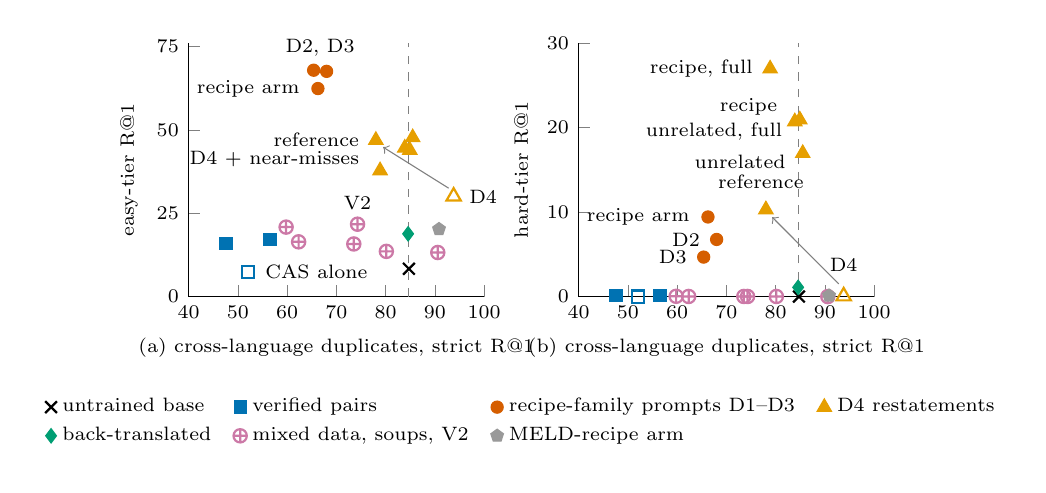
\begin{tikzpicture}
\begin{axis}[
  name=left,
  width=0.44\linewidth, height=4.8cm,
  xmin=40, xmax=100, ymin=0, ymax=76,
  xtick={40,50,60,70,80,90,100}, ytick={0,25,50,75},
  xlabel={(a) cross-language duplicates, strict R@1}, ylabel={easy-tier R@1},
  label style={font=\scriptsize}, tick label style={font=\scriptsize},
  axis y line*=left, axis x line*=bottom, clip=false,
]
\addplot[gray, dashed, forget plot] coordinates {(84.73,0) (84.73,76)};
\addplot[forget plot, only marks, mark=x, mark size=3pt, thick, black] coordinates {(84.73,8.32)};
\addplot[forget plot, only marks, mark=square*, mark size=2.2pt, cVer] coordinates {(56.52,17.05) (47.58,15.92)};
\addplot[forget plot, only marks, mark=square, mark size=2.2pt, thick, cVer] coordinates {(52.08,7.42)};
\addplot[forget plot, only marks, mark=*, mark size=2.2pt, cRec] coordinates {(66.26,62.38) (68.02,67.54) (65.39,67.88)};
\addplot[forget plot, only marks, mark=triangle, mark size=3pt, thick, cD4] coordinates {(93.81,30.03)};
\addplot[forget plot, only marks, mark=triangle*, mark size=3pt, cD4] coordinates {(78.02,46.91) (83.89,44.59) (78.88,37.79) (85.50,47.69) (84.91,43.93)};
\addplot[forget plot, only marks, mark=diamond*, mark size=2.6pt, cBT] coordinates {(84.57,18.81)};
\addplot[forget plot, only marks, mark=oplus, mark size=2.4pt, thick, cMix] coordinates {(74.30,21.70) (59.80,20.83) (80.15,13.55) (73.54,15.77) (62.34,16.41) (90.59,13.21)};
\addplot[forget plot, only marks, mark=pentagon*, mark size=2.4pt, cMELD] coordinates {(90.84,20.23)};
\draw[->, thin, gray] (axis cs:92.8,32.5) -- (axis cs:79.5,44.8);
\node[font=\scriptsize, anchor=east] at (axis cs:64.5,62.38) {recipe arm};
\node[font=\scriptsize, anchor=south] at (axis cs:66.7,69.0) {D2, D3};
\node[font=\scriptsize, anchor=west] at (axis cs:95.0,30.03) {D4};
\node[font=\scriptsize, anchor=east] at (axis cs:76.6,46.91) {reference};
\node[font=\scriptsize, anchor=east] at (axis cs:76.6,41.2) {D4 + near-misses};
\node[font=\scriptsize, anchor=south] at (axis cs:74.30,23.2) {V2};
\node[font=\scriptsize, anchor=west] at (axis cs:53.6,7.42) {CAS alone};
\end{axis}
\begin{axis}[
  name=right,
  at={(left.south east)}, anchor=south west, xshift=1.2cm,
  width=0.44\linewidth, height=4.8cm,
  xmin=40, xmax=100, ymin=0, ymax=30,
  xtick={40,50,60,70,80,90,100}, ytick={0,10,20,30},
  xlabel={(b) cross-language duplicates, strict R@1}, ylabel={hard-tier R@1},
  label style={font=\scriptsize}, tick label style={font=\scriptsize},
  axis y line*=left, axis x line*=bottom, clip=false,
  legend to name=invfulllegend, legend columns=4, legend cell align=left,
  legend style={font=\scriptsize, draw=none, /tikz/every even column/.append style={column sep=6pt}},
]
\addplot[gray, dashed, forget plot] coordinates {(84.73,0) (84.73,30)};
\addplot[only marks, mark=x, mark size=3pt, thick, black] coordinates {(84.73,0.00)};
\addlegendentry{untrained base}
\addplot[only marks, mark=square*, mark size=2.2pt, cVer] coordinates {(56.52,0.16) (47.58,0.16)};
\addlegendentry{verified pairs}
\addplot[forget plot, only marks, mark=square, mark size=2.2pt, thick, cVer] coordinates {(52.08,0.00)};
\addplot[only marks, mark=*, mark size=2.2pt, cRec] coordinates {(66.26,9.42) (68.02,6.76) (65.39,4.67)};
\addlegendentry{recipe-family prompts D1--D3}
\addplot[only marks, mark=triangle*, mark size=3pt, cD4] coordinates {(78.02,10.30) (83.89,20.71) (78.88,26.97) (85.50,16.96) (84.91,20.93)};
\addlegendentry{D4 restatements}
\addplot[forget plot, only marks, mark=triangle, mark size=3pt, thick, cD4] coordinates {(93.81,0.04)};
\addplot[only marks, mark=diamond*, mark size=2.6pt, cBT] coordinates {(84.57,1.09)};
\addlegendentry{back-translated}
\addplot[only marks, mark=oplus, mark size=2.4pt, thick, cMix] coordinates {(74.30,0.01) (59.80,0.03) (80.15,0.01) (73.54,0.01) (62.34,0.01) (90.59,0.00)};
\addlegendentry{mixed data, soups, V2}
\addplot[only marks, mark=pentagon*, mark size=2.4pt, cMELD] coordinates {(90.84,0.11)};
\addlegendentry{MELD-recipe arm}
\draw[->, thin, gray] (axis cs:92.8,1.5) -- (axis cs:79.3,9.4);
\node[font=\scriptsize, anchor=east] at (axis cs:64.5,9.42) {recipe arm};
\node[font=\scriptsize, anchor=east] at (axis cs:66.6,6.76) {D2};
\node[font=\scriptsize, anchor=east] at (axis cs:63.9,4.67) {D3};
\node[font=\scriptsize, anchor=south] at (axis cs:93.81,1.8) {D4};
\node[font=\scriptsize, anchor=south] at (axis cs:77.0,11.6) {reference};
\node[font=\scriptsize, anchor=east] at (axis cs:77.3,26.97) {recipe, full};
\node[font=\scriptsize, anchor=east] at (axis cs:82.3,22.5) {recipe};
\node[font=\scriptsize, anchor=east] at (axis cs:83.3,19.5) {unrelated, full};
\node[font=\scriptsize, anchor=east] at (axis cs:84.0,15.9) {unrelated};
\end{axis}
\node[anchor=north, yshift=-4pt] at (current bounding box.south) {\pgfplotslegendfromname{invfulllegend}};
\end{tikzpicture}
\caption{The full plot behind Figure~\ref{fig:inversion}: every $0.6$B model of Tables~\ref{tab:controlled}, \ref{tab:dose-full}, \ref{tab:factorial} and~\ref{tab:mixing}, with the corrected-gate retrains and V2's no-instruction reading omitted. Same axes and conventions as Figure~\ref{fig:inversion}: horizontal, strict R@1 on cross-language duplicates, the dashed line and $\times$ the untrained base; colour, what the positives are; hollow, no negatives; the labels on the D4 cells name the negatives attached (``recipe'' and ``unrelated'' are LLM near-misses from the recipe's prompt and from an unrelated one, ``full'' at the recipe arm's negative volume). Two groups appear here only: the verified squares also include computer-algebra positives with no negatives (CAS alone) and the uncapped verified arm, and the crossed circles are the mixed-data, soup and V2 models of Appendix~\ref{sec:forgetting}, which sit near the hard-tier floor. The MELD-recipe arm is seed $42$ ($20.23$ easy, $0.11$ hard, $90.84$ real; Section~\ref{sec:ood}). (a)~Easy tier: every model trained on LLM rewrites scores above the verified ones. (b)~Hard tier: only deep LLM rewrites paired with negatives reach it; the arrow is the edit from D4 alone to the reference, attaching verified negatives, which lifts hard R@1 off the floor and costs $15.79$ retention points, and LLM-written near-misses lift the same restatements further (Table~\ref{tab:factorial}). Computer-algebra positives with the recipe's near-misses lie off the axis at $12.47$ real.}
\label{fig:inversion-full}
\end{figure}


\paragraph{Positives or negatives alone stay at the floor; together they match the recipe arm.}
Table~\ref{tab:factorial} gives the cells. Neither half of a pair does anything on the hard tier by itself: CAS positives score $0.00$ without negatives and $0.16$ with them, and D4's restatements score $0.04$ without. Put D4's restatements together with the CAS negatives and the model, the reference, reaches $10.30 \pm 1.15$ over eight seeds ($10.81$, $11.85$, $10.25$, $9.01$, $10.13$, $10.34$, $8.49$, $11.55$). That is level with the recipe arm's $9.42$ (recipe minus reference $-0.88$ $[-1.85, 0.10]$), ahead in seven of eight seed-paired comparisons ($+1.44$, $+1.10$, $+0.67$, $+0.02$, $+1.10$, $+1.42$, $-0.57$, $+1.86$) and clearly ahead at R@5 ($60.05$ against $57.20$; $-2.86$ $[-4.01, -1.67]$), with fewer negatives per row ($1.28$) than either controlled arm ($1.52$ and $2.63$). Nothing in that training file comes from the Appendix-F prompt: the positives are D4's restatements under an unrelated prompt (Appendix~\ref{app:prompts}) and the negatives are SymPy counterexamples. What the hard tier rewards is therefore the shape of the pair, a deep LLM rewrite against a hard negative, and not the words of the template's positives (Section~\ref{sec:mechanism}); the near-copy and back-translated cells below, whose positives are shallow, stay near the floor, which is why the positive has to be a deep LLM rewrite.

\paragraph{A count-matched cell and a full cell hold the positives fixed and swap the negatives' provenance.}
These two cells ask whether it matters who wrote the negatives, separately from how many there are (\texttt{scripts/build\_llmnegs\_cells.py}; readings registered as R6-a/b in \texttt{scripts/factorial\_cells.slurm} before any number existed). Each D4 row whose source problem also has a recipe-arm row takes that row's Appendix-F near-misses. The count-matched cell takes only the first $k$ of them, $k$ being the number the same source carries in the reference file, so the count stays close and only the origin changes: $5{,}978$ rows at $1.20$ negatives per row against the reference's $1.28$, the recipe arm's cap of three truncating $449$ rows. The full cell takes all of them, $2.64$ per row, the recipe arm's own volume. The $790$ D4 sources with no recipe-arm row are dropped, so both cells train on $2.7\%$ fewer rows than the reference. The registered reading: a count-matched cell within $2\sigma_1 = 1.72$ hard-tier points of the reference's then three-seed mean would mean the negatives' origin does not matter, more than $1.72$ above it would mean the recipe's near-misses add a recipe-specific increment, and more than $1.72$ below it would have meant verified negatives are the better half; a full cell at or above the recipe arm's $9.90$ less $1.72$ would mean the claim that the template's positives are not required survives.

\paragraph{The recipe's own near-misses beat counterexamples by ten points at matched count.}
Both cells landed far above their registered bands. The count-matched cell scores $20.71 \pm 0.82$ hard R@1 ($20.31$, $21.65$, $20.17$), $9.50$ to $9.92$ above the reference seed for seed and $10.59$ to $10.94$ above the recipe arm: swapping CAS counterexamples for the recipe's own near-misses, at the same count, doubles the hard-tier score, so under the registered reading the negatives' origin matters, with the unrelated-prompt cells below refining how much of that is specific to the recipe. The full cell scores $26.97 \pm 0.97$ ($26.47$, $28.09$, $26.35$), $17.55$ above the recipe arm's eight-seed mean at the recipe arm's own negative volume, so the claim that the template's positives are not required survives. The hard tier's recipe-sensitive part therefore lives in its negatives: near-misses written by the recipe's prompt, the genre of the benchmark's own distractors, beat SymPy counterexamples by ten points at matched count, of which the recipe's prompt itself accounts for $3.75$ (the unrelated-prompt cells below), while the template's positives are not required and are outscored by restatements from an unrelated prompt.

\paragraph{More near-misses cost easy-tier and retention points, and two limits travel with the reading.}On the easy tier the two LLM-negative cells score $44.59$ and $37.79$, both below the reference's $46.91$, and on real duplicates $83.89 \pm 3.82$ and $78.88 \pm 2.33$ against its $78.02$. So adding more of the recipe's near-misses buys hard-tier points and pays for them in easy-tier and retention points, and at matched count those near-misses cost less retention than the counterexamples do. Two caveats go with the reading: each new cell has three seeds, and the count-matched cell carries $0.08$ fewer negatives per row than the reference, a difference that works against it rather than for it. A third, that both cells draw their near-misses from the recipe's own prompt, is what the next cells test.

\paragraph{Near-misses from an unrelated prompt recover most of the negatives' effect; the recipe's prompt adds an increment.}
The third pair of cells asks whether the ten-point jump came from the recipe's prompt specifically or from LLM-written near-misses in general. A new prompt unrelated to the benchmark's Appendix-F template, keeping D4's audience persona and adding a ``spot the difference'' drill, wrote near-misses for D4's positives, with the ladder's generator, judge pass, seed and source problems (\texttt{scripts/gen\_unrelated\_negs.slurm}, \texttt{scripts/build\_review2\_cells.py}). Both cells hold the same $6{,}393$ rows ($285$ D4 sources had no such row and $90$ no surviving negative), of which $6{,}145$ train per seed; one is count-matched to the reference by the same rule as the recipe-negative cell ($1.20$ negatives per row), the other carries all of the new prompt's near-misses ($2.66$ per row). Every verdict file was regenerated in one pass after the last cell landed. The reading was registered before the cells trained (\texttt{scripts/factorial\_cells.slurm}, R7-a/b): within $2\sigma_1 = 1.72$ hard-tier points of the recipe's near-misses, LLM-written near-misses of any origin would be the potent half and ``recipe-specific'' would be retired for the negatives; more than $1.72$ below, the recipe's prompt adds an increment of its own, to be reported with its size. The second branch landed: $16.96 \pm 2.08$ hard R@1 ($14.67$, $18.73$, $17.48$) against the recipe near-misses' $20.71$ at matched count, a gap of $3.75$ $[1.83, 5.97]$, and $20.93 \pm 0.44$ against $26.97$ at full volume, a gap of $6.03$ $[5.01, 7.18]$ (nested bootstrap over queries and seeds, \texttt{results/reference\_control\_did.json}). The negatives' effect therefore breaks into three steps, CAS counterexamples $10.30$, an unrelated prompt's LLM near-misses $16.96$, the recipe's own $20.71$: most of the climb above verified negatives comes from the near-misses being LLM-written at all, and the recipe's prompt adds about a fifth of the count-matched score on top.

\paragraph{The unrelated prompt's near-misses score higher on the easy tier and leave cross-language retention at the base.}
The unrelated-prompt cells beat the recipe-negative cells on the easy tier ($47.69$ and $43.93$ against $44.59$ and $37.79$) and leave cross-language retention at the untrained base ($85.50 \pm 1.67$ and $84.91 \pm 1.49$ against $84.73$). At full volume, the extra hard-tier points the recipe's near-misses buy therefore come at a retention cost $6.02$ $[2.00, 10.18]$ cross-language points higher than the unrelated prompt's, which cost nothing; at matched count the two kinds of near-misses are within noise of each other on retention ($1.61$ $[-2.93, 6.22]$). On same-language reprints they are within noise too ($50.13$ against $47.73$ at matched count and $45.33$ against $39.47$ at full volume, the $45.33$ coinciding with the headline gap's value by chance; Table~\ref{tab:samelang}). The caveat that remains is that all the unrelated near-misses come from one prompt and one generator.

\paragraph{Near-copy positives with the recipe's near-misses stay at the floor and lose the most retention of any cell.}
One suspect for the verified arm's cross-language collapse is its counterexampled negatives: tiny notational edits might teach the model to fixate on notation. The cell that tests this keeps the verified arm's near-copy positives (one seeded CAS row per source) and swaps in the recipe arm's own near-misses, all of them ($6{,}145$ rows, $2.63$ per row; \texttt{build\_review2\_cells.py -{}-which r8}). Two readings were registered (R8-a/b): more than $1.72$ hard-tier points above the verified arm's $0.16$ would mean the recipe's near-misses lift even near-copy positives, and more than $6.54$ cross-language points ($2\sigma_1$ for that set) above the verified arm's $56.52$ would make the counterexamples the driver of the collapse. Neither happened. Hard R@1 is $0.11 \pm 0.03$ ($-0.05$ $[-0.13, 0.03]$ against the verified arm): the tier needs the deep-rewrite positive too, not only the right negatives. Cross-language retention fell to $12.47 \pm 0.68$, $44.05$ $[38.62, 49.34]$ points \emph{below} the verified arm and outside both registered branches. Replacing the counterexamples made the collapse worse, so they are not its driver, and near-copy positives set against the recipe's near-misses are the most destructive pairing we trained ($12.47$; only the pure SABER document channel's $10.69$ is lower). The same-language primary slice falls to $34.40$ ($-16.90$ $[-24.08, -10.06]$ against the verified arm) and the easy tier to $11.28$.

\paragraph{Back-translated positives: the non-LLM paraphrase control.}
The reference's $29.85$-point gain over the verified arm mixes two things, deep paraphrase and LLM authorship, because every deep paraphrase in the paper is LLM-written. The control separates them with a paraphrase no LLM wrote: each source problem is translated out and back through NLLB-200-distilled-600M, a dedicated machine-translation model rather than a general-purpose LLM (English through French and back, other languages through English; LaTeX spans masked and restored; no LLM judge), and paired with the reference's own counterexampled negatives (\texttt{scripts/backtranslate\_anchors.py}; $6{,}576$ rows, $1.26$ negatives per row; $186$ round trips came back identical to the source and $6$ failed a structural check, all dropped). The paraphrase is real but shallower than a free restatement: character-$3$-gram Jaccard to the source $0.783$ (median $0.797$), between the verified arm's $0.865$ and D4's $0.421$. Registered reading (R9): within $2.40$ easy-tier points of the reference, LLM authorship would not matter for the genre share; more than $2.40$ below, LLM authorship carries part of the reference's gain, reported as reference minus back-translation. It landed far below: $18.81 \pm 0.80$ easy R@1, $28.10$ $[26.74, 29.51]$ under the reference and only $1.76$ $[0.62, 2.82]$ above the verified arm, with $1.09 \pm 0.04$ hard R@1 ($0.93$ $[0.76, 1.10]$ above the verified arm). A non-LLM paraphrase covering the first $0.08$ of the character-overlap distance from the verified arm's positives toward D4's buys $1.76$ of the $29.85$ points; for depth alone to explain the share, the remaining $0.36$ of that distance would have to buy the other $28$. Depth and authorship are therefore separated down to the control's depth, and no further (Section~\ref{sec:limitations}). A second result rides on the same cell: with the very negatives that cost D4's restatements $15.79$ cross-language points, the back-translated positives sit at the base on both probes ($84.57 \pm 1.20$ cross-language against $84.73$; $57.87$ same-language against $62.40$, $-4.53$ $[-14.09, 5.07]$), so what the negatives cost in retention depends on the positives they are paired with. Trained alone, the back-translated positives score $12.92 \pm 0.72$ on the easy tier against D4's $30.03$ and D5's $18.71$ alone, the same authorship gap with no negatives in play, and $94.57 \pm 0.64$ on cross-language duplicates, the highest of all our models (Table~\ref{tab:factorial}).

\paragraph{A second recipe-free prompt recovers less of the easy-tier gap, so the recipe-specific share is a range.}
One objection is that the recipe-specific share might rest on a single recipe-free prompt: if D4 were an unusually retention-friendly prompt rather than the recipe family an unusually gaming one, the $15.47$-point attribution and the $27.24$ difference-in-differences would move with the prompt. We therefore wrote a second recipe-free restatement prompt, D5, framed differently from D4's audience change: a survey author restating another author's problem for a themed collection in their own wording, notation and order, level and mathematics unchanged, positives only (\texttt{scripts/gen\_survey.slurm}; same generator, judge pass, source problems and seed as the ladder; $6{,}293$ verified positives of $7{,}089$ sources, $698$ generation failures, $98$ judge rejections). D5's positives are slightly closer to their anchors than D4's (character-$3$-gram Jaccard $0.472$ against D4's $0.421$ and D1's $0.463$). Two cells were trained, three seeds each: D5 alone, and D5 with the reference's own counterexampled negatives per source, which we call the D5 reference (the main text's reference is the D4 reference here; \texttt{build\_review2\_cells.py -{}-which r10}; $6{,}163$ rows, $1.28$ negatives per row, $605$ D4 sources without a verified D5 positive dropped). Three readings were registered (\texttt{scripts/factorial\_cells.slurm}, R10-a/b/c). First, the recipe arm's easy-tier lead over the D5 reference within $2.40$ of the $15.47$ lead over the D4 reference would mean the share does not depend on the prompt, and further away would make it a range over both references. Second, the D5 cells within $6.54$ of their D4 counterparts' cross-language retention would mean D4 is not unusually retention-friendly. Third, the D5 reference within $1.72$ of the D4 reference's $10.30$ hard R@1 would replicate ``recipe-free rewrites with verified negatives reach the tier''. Outcomes: D5 alone scores $18.71 \pm 1.31$ easy R@1 against D4's $30.03$ at the same cross-language retention ($93.72 \pm 0.39$ against $93.81$), and the D5 reference $39.20 \pm 0.40$ easy, $3.97 \pm 1.05$ hard ($3.50$, $5.17$, $3.24$) and $78.71 \pm 0.59$ cross-language against the D4 reference's $46.91$ / $10.30$ / $78.02$. R10-a: the recipe arm leads the D5 reference by $23.18$ $[22.10, 24.23]$ easy-tier points (nested bootstrap as in the reference contrasts, third random stream, \texttt{results/reference\_control\_did.json}), $7.71$ more than the $15.47$ against the D4 reference and outside the band, so the recipe-specific share is reported as a range, $15.47$ to $23.18$ at verified negatives ($24.59$ at matched LLM negatives, below), and the difference-in-differences against the D5 reference is $35.63$ $[29.69, 41.41]$ against $27.24$. R10-b: both D5 cells retain what their D4 counterparts retain on cross-language duplicates ($+0.69$ $[-1.84, 3.16]$ and $-0.09$), so D4 is not unusually retention-friendly; the two prompts differ in how much of the easy tier they recover, not in what they keep. R10-c: the D5 reference is $6.33$ $[4.99, 7.54]$ hard-tier points below the D4 reference, outside the band, so the hard-tier level a recipe-free reference reaches depends on the restatement prompt; the verified negatives still lift D5 from $0.01$ to $3.97$, $3.81$ $[2.98, 4.90]$ above the verified arm. In the paper's terms, the recipe-free share of the easy-tier gap is $22.15$ $[21.06, 23.21]$ of $45.33$ points with D5 and $29.85$ with D4, half to two thirds, the range the abstract and Section~\ref{sec:gaming} carry. On same-language reprints D5 alone sits at the base ($64.53$ against $62.40$, within noise) and the D5 reference at $41.33$, beside the D4 reference's $39.20$ (Table~\ref{tab:samelang}).

\paragraph{Writing positives and near-misses in separate calls leaves the recipe arm's hard tier where it was.}
Why do D4's restatements beat the recipe's own positives on the hard tier when both get the recipe's near-misses? Three accounts are listed below, and we tested the first: that a positive and its near-misses written in one LLM call share phrasing, so the model learns to key on subtler features and gets less from the positive. We cut the Appendix-F prompt by string surgery into a positives-only call and a near-misses-only call, every surviving line verbatim D1's, with the judge pass, sources and seed unchanged (\texttt{scripts/gen\_split.slurm}, variant \texttt{exact\_split}; $6{,}516$ verified positives and $18{,}080$ verified near-misses, $2.61$ per row, $6{,}145$ rows trained per seed; the split-call positives sit at character-$3$-gram Jaccard $0.430$ to the anchor against the one-call arm's $0.463$). Registered (R11-a): within $1.72$ hard-tier points of the recipe arm's $9.42$, the one-call pairing is not what holds the recipe arm's hard tier down; more than $1.72$ above, the shared-phrasing account holds. It landed within the band, $9.79 \pm 0.66$ ($+0.37$ $[-0.41, 1.22]$), so the account is not supported. The split-call arm also stays $17.18$ points below D4's restatements under the recipe's own near-misses (R11-b), so which prompt writes the positives matters at those negatives whether or not the calls are separated. Separating the calls has costs, $3.91$ $[2.63, 5.28]$ easy-tier points ($58.47 \pm 1.18$), $14.18$ $[10.08, 18.40]$ cross-language points ($52.08 \pm 1.49$) and $9.77$ same-language points ($36.53$), and one gain, the medium tier rising to $12.37 \pm 0.49$ from the recipe arm's $8.84$ (R11-c, reported without a registered direction). Two accounts remain untested: that D4's restatements are written in a different register, and that D4's audience-change framing acts as a regularizer.

\paragraph{A second, independent judge leaves the recipe arm's easy-tier score in place, lowers its hard tier a little and raises its retention.}
The recipe arm's judge is the same model that generated its pairs, where the benchmark uses two independent judges. To see whether that matters, every candidate row of the recipe arm's generation ($25{,}656$) was re-judged by Mistral-Small-24B-Instruct-2501, a different vendor and model family, under the same judge prompt (\texttt{scripts/rejudge.slurm}; \texttt{generate\_llm\_pairs.py -{}-rejudge-input}), and a cell was trained on the rows both judges admit. Agreement (R12-a): of $6{,}414$ candidate positives the self-judge accepts $6{,}145$ and the second judge $5{,}522$; both accept $5{,}398$, only the first $747$, only the second $124$, neither $145$ (agreement $0.864$, but Cohen's $\kappa$ only $0.198$, since nearly everything is accepted and most agreement is by chance); of $19{,}242$ near-misses both accept $16{,}107$ (agreement $0.879$, $\kappa$ $0.346$); $1{,}110$ second-judge verdicts did not parse and count as not verified. The two-judge file has $5{,}398$ rows, below the $6{,}145$ budget, so the cell trains on all of them ($2.53$ negatives per row; positives at Jaccard $0.460$). Registered (R12-b): within $2.40$ easy, $1.72$ hard and $6.54$ cross-language points of the recipe arm, its numbers do not depend on the single self-judge; outside any band, the size is reported and Section~\ref{sec:setup} discloses the arm as single-judge. Outcomes over three seeds: easy $64.71 \pm 0.64$, $+2.33$ $[1.47, 3.25]$, inside the band; hard $7.58 \pm 0.39$, $-1.84$ $[-2.42, -1.27]$, just outside it; cross-language $74.81 \pm 2.65$, $+8.56$ $[4.85, 12.34]$, outside it in the arm's favour; same-language $46.13$ against $46.30$. The easy-tier headline therefore does not depend on the self-judge, while a stricter second judge trims the hard tier and gives back nearly half of the arm's cross-language loss ($8.56$ of the $18.47$ points it sits below the base).

\paragraph{Three back-translation hops deepen the non-LLM paraphrase but recover none of the reference's gain.}
Does the LLM-authorship attribution hold at a non-LLM paraphrase depth beyond the single hop's $0.783$? We ran the back-translation of the previous control three times in sequence (\texttt{scripts/bt2.slurm}: French, then German, then Russian, with English substituted for any pivot equal to the source language; formulas masked at every hop; a row kept only if every hop validates). $5{,}723$ of $6{,}768$ source problems survive ($1{,}038$ came back identical to the source after the chain, $7$ failed a structural check), at character-$3$-gram Jaccard $0.640$ to the source (median $0.644$), between the single hop and D4's $0.421$; the cell keeps the reference's negatives ($1.21$ per row). Registered (R13): within $2.40$ easy-tier points of the reference's $46.91$, deeper non-LLM paraphrase recovers the reference's gain and the attribution is retired; more than $2.40$ below, it survives to the deeper depth. It landed at $12.85 \pm 0.56$, $34.06$ $[32.81, 35.41]$ below the reference, below even the single-hop cell's $18.81$ and $4.21$ $[3.25, 5.15]$ below the verified arm, with $4.47 \pm 0.15$ hard R@1, $67.01 \pm 1.73$ cross-language ($11.02$ $[5.20, 16.94]$ below the reference) and $46.67$ same-language. The attribution survives, with a caveat the reading needs: three translation hops degrade the text rather than restate it, since a sixth of the rows return unchanged and the rest lose fluency, and the model loses retention with them. The added depth is therefore noise depth, not restatement depth, and this control bounds the depth account no more tightly than the single hop did. The hard tier reads the same event the other way round: with the negatives unchanged, the noisier positive lifts hard R@1 from $1.09$ to $4.47$, so what the tier pays for is the positive's distance from its minimal-edit near-miss, which translation noise supplies as well as a deep rewrite does, and not equivalence, which the noise can only degrade.

\paragraph{The remaining cells of the grid.}Seven further cells completed the grid of Table~\ref{tab:design}, built from existing positive and negative files with the grid's own conventions (computer-algebra negatives are the reference's per source; LLM near-misses are all of the partner row's, the recipe arm's volume; \texttt{scripts/build\_review4\_cells.py}), three seeds each, with no directional prediction registered (Table~\ref{tab:factorial}). Three things they add. First, positives trained alone never register on the hard tier, whoever wrote them: the recipe's own positives without negatives score $0.00$, back-translations $0.05$, beside D4's $0.04$ and D5's $0.01$; and paraphrase positives alone, LLM-written or back-translated, sit at the top on cross-language duplicates ($94.57$ for back-translations, $93.81$ for D4, $93.72$ for D5, within noise of one another), where the recipe's positives alone stay near the base ($83.21$). Second, LLM near-misses need a deep LLM rewrite to work with: on near-copy positives they reach $0.23$ hard R@1 from an unrelated prompt and $0.11$ from the recipe's, on back-translated positives $1.88$ and $4.18$, against $16.96$ to $26.97$ on D4's restatements, and in every one of these four cells cross-language retention collapses, to between $12.47$ and $38.67$, whichever prompt wrote the near-misses; the collapse follows the pairing of LLM near-misses with shallow positives, not the recipe's negatives in particular. Third, the recipe's own positives with the reference's negatives score $50.25$ easy, $2.09$ hard and $70.82$ cross-language, against the reference's $46.91$, $10.30$ and $78.02$ with the same negatives: the template's positives buy $3.34$ easy-tier points over D4's at verified negatives, reach a fifth of the reference's hard-tier score and lose $7.20$ more cross-language points; against the recipe arm itself ($62.38$, $9.42$, $66.26$), swapping its near-misses for verified negatives removes $12.13$ easy and $7.33$ hard points and returns $4.56$ cross-language points, so on the easy tier the recipe's near-misses help its own positives where they hurt D4's. One number we report without an account: D1 positives with an unrelated prompt's near-misses score $20.51 \pm 1.52$ on the medium tier ($22.22$, $19.31$, $20.01$), more than twice any other model we trained (the recipe arm $8.84$).

\paragraph{What this changes in the ladder's reading, and what it leaves standing.}The ladder's registered decay prediction passed and its numbers stand, but two of its steps now mean less than they seemed to. The D3-to-D4 drop ($4.67 \to 0.04$) is D4's missing negatives, not its prompt: D4's positives reach $10.30$ with the verified arm's negatives and $26.97$ with the recipe arm's. And within D1--D3 the ladder cannot tell whether the decline comes from the positives' wording or from the near-misses' quality, because each of those prompts writes both. What the ladder still shows on its own is a hard-tier decline across D1--D3, whichever mix drives it, and the exact template scoring lowest of the three on the easy tier. The two claims about the hard tier, that the template's positives are not needed and that its near-misses add an increment over an unrelated prompt's, are the factorial's results, not the ladder's.

\paragraph{The easy tier stays genre-level, and the verified arm's gain rides on its negatives.}Two easy-tier facts from the factorial. Attaching CAS negatives to D4's restatements lifts their easy R@1 from $30.03$ to $46.91$, still $15.47$ points below the recipe arm's $62.38$, so the genre reading of Section~\ref{sec:mechanism}, LLM-rewrite genre with a recipe-specific remainder on top, stands. The opposite corner of the grid runs the other way: CAS positives without negatives score $7.42$, below the untrained base's $8.32$, so everything the verified arm gains on the easy tier over the base ($8.32$ to $17.05$) comes from its counterexampled negatives, not its positives.

\paragraph{The two negative-free cells diverge by a cross-lingual loss whose cause is open.}
The two cells trained without negatives behave very differently on cross-language duplicates: D4's restatements alone reach $93.81$ strict R@1, above the untrained base, while CAS positives alone fall to $52.08$. On same-language reprints the two sit at the base together ($61.07$ and $58.13$; Appendix~\ref{app:setup}), so the difference is specifically about working across languages, not about recognising equivalent problems. Which property of D4 preserves that ability the factorial cannot say. Two candidates: D4's rows cover more source problems ($6{,}145$ against $4{,}621$ for the verified arm's draw at the same seed), and its prompt asks for a change of audience rather than an equivalence-preserving disguise, which may act as a regularizer the way V2's instruction does. Telling them apart would need a D4 trained on the verified arm's sources and a verified arm trained under an audience-change instruction, neither of which we have built.

\paragraph{Why the recipe's positives lose to D4's at fixed LLM negatives is open.}
Keep the recipe arm's own near-misses and swap its positives for D4's restatements: hard R@1 rises from $9.42$ to $26.97$ and cross-language retention from $66.26$ to $78.88$. The same holds at verified negatives: D1's positives with the reference's counterexamples reach $2.09$ where D4's reach $10.30$, and $70.82$ cross-language where D4's reach $78.02$ (Table~\ref{tab:factorial}). Why should another prompt's positives beat the benchmark's own? Three accounts fit the data. First, the recipe writes each positive and its near-misses in one call under one prompt, so they share phrasing, and the contrastive task must key on subtler features than when the positive comes from another prompt. Second, D4's audience-change restatements sit farther from the anchor in register, a deeper paraphrase against the same near-miss. Third, as the previous paragraph suggested for retention, the audience-change framing may act as a regularizer. The first was tested and is not supported: written in separate calls, the recipe's positives and near-misses leave its hard tier where it was ($9.79$ against $9.42$; above). The other two remain untested. Style tracking (Table~\ref{tab:style}) does not decide between them: the models trained on D4's positives carry little of the recipe fingerprint whether their negatives are verified or the recipe's own (the unrelated-prompt cells were not scored). Separating the remaining two would need a verified arm trained under an audience-change instruction, which we have not built.

\paragraph{The inversion under a single edit to the training file.}
Start from D4's restatements alone, at $93.81$ strict R@1 on cross-language duplicates, first among our trained models. Attach the verified negatives and the hard tier rises to $10.30$ while retention falls $15.79$ points to $78.02$, from first place to $6.71$ below the untrained base. Attach the recipe's near-misses instead and retention falls $9.92$ at matched count ($83.89$) and $14.93$ at full volume ($78.88$), for $20.71$ and $26.97$ hard R@1; on same-language reprints the verified negatives and the recipe's near-misses cost $13$ to $22$ points and an unrelated prompt's $11$ to $16$ (Table~\ref{tab:samelang}). Attach an unrelated prompt's near-misses and the cross-language cost is $8.31$ or $8.90$ points ($85.50$, $84.91$), which leaves the model at the untrained base. In every case a single edit that touches no positive and no prompt, only the negatives, lifts the hard tier and lowers retention from D4's $93.81$.

\paragraph{The recipe arm against the reference: the recipe-specific share, and how much of each step transfers.}
The reference, not the verified arm, is the comparison that isolates the recipe-specific share of the gap, and Table~\ref{tab:controlled} reads the headline gaps against both. The intervals come from \texttt{scripts/reference\_control\_did.py}, a nested bootstrap ($B = 5{,}000$) that resamples easy-tier queries and duplicate clusters paired across arms and each arm's eight training seeds independently. Recipe minus reference: $+15.47$ $[14.11, 16.73]$ on the easy tier and $-11.77$ $[-17.33, -6.09]$ on cross-language duplicates, so the gap shrinks by $27.24$ $[21.40, 32.93]$ from benchmark to real data, positive in every replicate and in each of the eight seed-paired comparisons ($24.75$ to $31.69$). Reference minus verified: $+29.85$ $[28.56, 31.15]$ easy-tier points, of which $+21.50$ $[15.31, 27.67]$ carry over to cross-language duplicates, so this gap shrinks by only $8.35$ $[1.93, 14.78]$. The two shrinkages sum to the published $35.59$ by construction. On the medium tier the recipe arm leads the reference by $4.62$ $[4.13, 5.15]$; on the hard tier the two are tied at R@1 ($-0.88$ $[-1.85, 0.10]$, an interval spanning zero) and the reference leads at R@5 ($-2.86$ $[-4.01, -1.67]$). On the same-language primary slice the recipe arm leads the reference by $7.10$ $[-2.34, 17.04]$, so the shrinkage there is $8.37$ $[-1.14, 18.16]$, both intervals spanning zero, while the reference trails the verified arm by $12.10$ (Table~\ref{tab:samelang}). The reference's real-data advantage over the recipe arm therefore shows up cross-lingually only.

\paragraph{The recipe-specific share at matched negatives.}
The reference carries the verified arm's counterexamples, so the $15.47$-point share compares training sets that differ in two ways, the positives' prompt and the negatives' origin. To isolate the prompt, compare the recipe arm with the D4 cells that carry the recipe's own near-misses (three seeds each; same bootstrap, separate random stream, \texttt{results/reference\_control\_did.json}). The recipe arm leads the count-matched cell by $17.79$ $[16.25, 19.38]$ easy-tier points and the full cell, which shares its negatives outright so that only the positives' prompt differs, by $24.59$ $[23.14, 26.29]$. On cross-language duplicates it trails them by $17.63$ $[12.21, 23.20]$ and $12.63$ $[7.51, 17.63]$, so the gap shrinks by $35.42$ $[29.56, 41.14]$ and $37.22$ $[32.00, 42.61]$ from benchmark to real data. On the hard tier it trails them by $11.29$ $[10.29, 12.37]$ and $17.55$ $[16.42, 18.81]$. The prompt buys more of the easy tier at LLM negatives than at verified ones because the counterexamples themselves lift the easy tier (the reference's $46.91$ against the LLM-negative cells' $44.59$ and $37.79$), and what it buys reaches neither duplicate probe: the same-language shrinkages are $19.22$ $[12.50, 25.47]$ and $17.76$ $[9.84, 25.14]$.

\paragraph{The style probe, and the artefacts stripped before fitting it.}The probe is a plain text classifier, a logistic regression over word $1$--$2$-gram tf-idf features. It is trained on matched pairs, each source problem's organic text against that same problem's Appendix-F rewrite, with the train/test split by source problem so that topic and language confounds cancel and only writing style is left to learn; on held-out problems it reaches $0.880$ AUC. Two formatting quirks of our organic corpus that exist nowhere in the benchmark are stripped before fitting and scoring: a leading ``\texttt{Problem:}'' OCR header ($63.88\%$ of organic anchors against $0.02\%$ of rewrites) and image placeholders ($4.01\%$ against $0.16\%$). Left in, they inflate the holdout AUC to $0.969$ while \emph{costing} cross-generator transfer, because the classifier learns our corpus's formatting rather than LLM style, so the stripped detector is the one reported throughout. Its heaviest weights (\texttt{results/style\_probe\_features.json}) say what the fingerprint is made of. On the rewrite side the top features are the register of a set exercise, the imperatives and connectives \emph{determine}, \emph{define}, \emph{let}, \emph{suppose}, \emph{show that}, \emph{where} and \emph{with} (coefficients $2.4$ to $6.1$), with two LaTeX habits beside them, the \texttt{\textbackslash text} macro and \texttt{\textbackslash sum} with a subscript; on the organic side they are \emph{we}, \emph{then}, \emph{so that}, \emph{find}, \emph{what}, \emph{which} and article phrases such as \emph{of the} and \emph{the triangle} ($-2.0$ to $-4.6$). The fingerprint is therefore mostly how the rewrites phrase and frame a problem, with macro standardisation a smaller second part, and nothing in it is mathematical content.

\paragraph{Cross-generator transfer is the load-bearing result.}The detector was trained only on our Qwen rewrites, yet it separates the benchmark's Gemini-3-flash gold rewrites, from a vendor whose text it never saw, from $1{,}668$ organic corpus problems at AUC $0.804$ ($0.807$ once the organic documents that also appear among the probe's training anchors are dropped; $0.778$ / $0.839$ / $0.796$ on the easy / medium / hard tiers). The fingerprint it learned is therefore a general LLM-rewrite fingerprint, not one specific to its own generator. The benchmark's minimal-edit near-miss distractors, which are small edits of organic problems and so inherit organic style, sit near chance ($0.562$), as they should.

\paragraph{The split caveat: $20$ held-out anchors have byte-identical training twins.}The probe's train/test split is by \emph{source id} rather than by text, and because some corpus problems appear under more than one id, $20$ of the $1{,}282$ held-out anchors have a byte-identical copy among the training negatives ($19$ on the rewrite side). At $1.6\%$ of the held-out set this cannot move the $0.880$ materially, but ``never seen in training'' would be the wrong words for it.

\begin{table}[htbp]
\centering
\caption{What the style detector detects. Each row takes one prompt's rewrites (held-out sources only) and gives the AUC with which the detector separates them from the same $1{,}282$ held-out organic problems, with $95\%$ CIs from $2{,}000$ bootstrap replicates over held-out source ids. The three recipe-family prompts D1--D3 are detected at about the same level and cannot be told apart within their intervals; the recipe-unrelated prompt D4 is detected far less strongly but still well above chance. The detector therefore mostly picks up the \emph{genre} of LLM rewrites, which D4 shares, plus a recipe increment of $0.204$ $[0.186, 0.222]$ that only the recipe-family prompts add.}
\label{tab:panel}
\small
\setlength{\tabcolsep}{4pt}
\begin{tabular}{@{}p{5.9cm}>{\centering\arraybackslash}p{2.2cm}>{\centering\arraybackslash}p{2.2cm}>{\centering\arraybackslash}p{2.8cm}@{}}
\toprule
Rewrite prompt & Held-out positives & AUC vs.\ organic & $95\%$ CI \\
\midrule
D1: the benchmark's Appendix-F template & $1{,}282$ & \textbf{0.8802} & $[0.8679, 0.8917]$ \\
D2: paraphrase of that template & $1{,}249$ & 0.8756 & $[0.8624, 0.8873]$ \\
D3: rewrite prompt in a different style & $1{,}096$ & 0.8654 & $[0.8520, 0.8788]$ \\
D4: restatement prompt unrelated to the recipe & $1{,}265$ & 0.6758 & $[0.6569, 0.6948]$ \\
\bottomrule
\end{tabular}
\end{table}

\paragraph{Genre with a recipe increment: what that costs the claim.}D4's prompt never mentions the recipe, yet against the same held-out organic anchors (Table~\ref{tab:panel}) its rewrites are still detected at $0.676$, so most of what the detector picks up is present in any LLM rewrite. The part specific to the recipe is the climb from D4 to D1, $0.204$ $[0.186, 0.222]$, positive in $100\%$ of bootstrap replicates. Within D1--D3 the detector resolves almost nothing: D1 $-$ D2 $= +0.005$ $[-0.006, 0.016]$ includes zero, and D1 $-$ D3 $= +0.015$ $[0.002, 0.027]$ excludes it but is a fourteenth of the D4-to-D1 climb, so the ladder of detectability inside the recipe family is at most a shallow one. That rules out the stronger characterization, ``a property of the recipe, not of the generator''. What the evidence supports is weaker: an LLM-rewrite genre signature that carries across generators, with a recipe increment on top.

\begin{table}[htbp]
\centering
\caption{Style tracking: does a model rate LLM-styled documents as more similar? For each of $2{,}000$ sampled queries against the full $117{,}088$-document corpus (single runs at seed $42$), the first column is the Spearman correlation between the model's similarity to each document and the artefact-stripped detector's style score for it, averaged over queries; positive means similarity rises with LLM style. The second column is where the model's top-$10$ documents sit in the corpus's style distribution, as a percentile, where $50$ means no preference (we report percentiles because the detector's raw score is an unbounded log-odds whose ratios have no scale meaning). The base and the verified arm show no style preference, D4's restatements alone none, and D4 with negatives of either kind only a faint one; the recipe-family prompts track clearly, in ladder order, with the exact template strongest.}
\label{tab:style}
\small
\setlength{\tabcolsep}{4pt}
\begin{tabular}{@{}p{7.4cm}>{\centering\arraybackslash}p{3.0cm}>{\centering\arraybackslash}p{3.0cm}@{}}
\toprule
Model & $\rho$(similarity, style) & Top-$10$ style percentile \\
\midrule
Base 0.6B (untrained) & $-0.061$ & 44.8 \\
Verified arm & $-0.019$ & 45.5 \\
D4: restatement prompt unrelated to the recipe & $-0.000$ & 48.1 \\
Reference (D4 $+$ CAS negatives) & $+0.025$ & 52.0 \\
D4 $+$ recipe-prompt near-misses, count-matched & $+0.046$ & 53.1 \\
D4 $+$ recipe-prompt near-misses, full & $+0.050$ & 53.5 \\
D3: rewrite prompt in a different style & $+0.105$ & 57.2 \\
D2: paraphrase of the benchmark's template & $+0.164$ & 61.6 \\
D1: the benchmark's template ($=$ recipe arm) & $\boldsymbol{+0.171}$ & \textbf{61.9} \\
\bottomrule
\end{tabular}
\end{table}

\paragraph{The recipe arm tracks the fingerprint; the verified arm does not.}Table~\ref{tab:style} correlates each model's similarity scores with the detector's style score over $2{,}000$ sampled queries against the full corpus. The untrained base mildly prefers documents that do \emph{not} look LLM-written ($\rho = -0.061$), the verified arm has no preference ($-0.019$), and the recipe arm prefers LLM-styled documents at $+0.171$, a $+0.190$ margin over the verified arm per query and higher on $94.20\%$ of queries (Wilcoxon $p < 10^{-308}$), so the difference is not carried by a few outliers. Seen from the retrieved side, the recipe arm's top-$10$ sits at the $61.9$th percentile of the corpus style distribution, where $50.0$ would be no preference, while the verified arm ($45.5$) and the base ($44.8$) retrieve slightly below-average-style documents.

\paragraph{The rungs scope the claim: the recipe's rewrite prompts as a family install it, not the template alone.}Is the tracking caused by the benchmark's exact prompt or by any prompt of its kind? Running the same statistic on the ladder rungs answers it (no new training was needed; their embedding caches existed). D2 tracks at $+0.164$, $96\%$ of the recipe arm's, D3 still at $+0.105$, and only D4, whose prompt never mentions the recipe, is flat ($-0.000$), matching the verified arm. We therefore claim that the recipe's rewrite prompts as a family install the tracking, more strongly the closer the prompt is to the template, and that neither D4's recipe-unrelated prompt nor verified training does. We do not claim that the template alone, or the recipe uniquely, installs it.

\paragraph{The reference and the recipe-negative cells track the fingerprint only faintly.}
Do the cells that score highest on the hard tier chase LLM style? The same statistic on the seed-$42$ models of the factorial's later cells (\texttt{scripts/style\_tracking\_review2.slurm}, cached embeddings, same detector) says barely: $+0.025$ for the reference, $+0.046$ for the count-matched cell with the recipe's near-misses and $+0.050$ for the full cell (top-$10$ percentiles $52.0$, $53.1$ and $53.5$), above D4's flat $-0.000$, below D3's $+0.105$, and a small fraction of the recipe arm's $+0.171$. Attaching verified negatives or the recipe's near-misses to D4's positives adds a little tracking (the unrelated-prompt cells were not scored); most of the recipe arm's tracking comes from its positives. The cells that buy the most hard-tier score ($20.71$ and $26.97$) therefore carry little of the fingerprint: whatever they learn to score on that tier, it is not style, and the probe does not explain it (Section~\ref{sec:limitations}).

\paragraph{The base-rate control: tracking survives within a single document class.}A pooled correlation over the whole corpus could be an artefact of ranking. The style score alone separates the benchmark's golds from its minimal-edit near-misses at AUC $0.750$, and the recipe arm is trained to rank golds above near-misses, so a correlation between similarity and style might only be picking up that ranking. Restricting to synthetic documents does not settle it: the correlation is unchanged ($+0.170$ vs.\ $-0.019$) but only $1.42\%$ of the corpus is removed, and the confound sits between the two synthetic classes. The test is to hold the class fixed. Within golds alone the recipe arm still tracks style, $\rho = +0.093$ against the verified arm's $-0.012$, and within near-misses alone $+0.086$ against $-0.009$ (\texttt{results/style\_within\_class.json}), roughly half the pooled margin. The tracking is therefore not an artefact of ranking golds above near-misses.

\paragraph{Hit accounting in full.}
On the hard tier the recipe arm alone ranks the gold first on $1{,}401$ of the $15{,}000$ queries and the verified arm alone on $15$ ($4$ both, $13{,}580$ neither). What makes those $1{,}401$ queries different: word overlap (token Jaccard) between query and gold separates them from the rest at AUC $0.639$ (means $0.21$ vs.\ $0.17$); overlap in \LaTeX{} spans separates them slightly ($0.557$); how densely the gold uses the recipe's phrasing and how LLM-styled it is do not separate them at all ($0.509$ and $0.511$, $p \ge 0.16$); and the gold/query length ratio runs weakly the \emph{opposite} way ($0.481$). The skew towards word overlap is a shifted distribution, not a rule: only $17.8\%$ of the wins fall among the $1{,}401$ queries with the highest overlap and $30.8\%$ sit below the median. The two probe-derived measures were computed with the pre-stripping detector; since both are null results, that does not matter.

\paragraph{Are published models already recipe-inflated? A pre-specified null.}The attack shows that a benchmark score can be inflated by training on pairs built like the benchmark's own, not that anyone has done so. To check the models actually on the leaderboard, we ran the same artefact-stripped detector on the same $2{,}000$-query sample over every public model whose corpus and query embeddings were already cached (\texttt{results/style\_probe\_public\_models.json}). As a check that the two runs are comparable, the untrained \texttt{base-0.6b} row gives the identical correlation ($-0.0610$) in both tables.

\begin{table}[htbp]
\centering
\caption{Do public models show the recipe-style signature? The same two measures as Table~\ref{tab:style}: $\rho$ is the mean per-query Spearman correlation between a model's query--document similarity and the document's LLM-style score, and the last column is where the model's top-$10$ documents sit in the corpus's style distribution, as a percentile, with $50$ meaning no preference. Every public model sits in the same narrow band as the untrained base and our verified arm, between $-0.07$ and $+0.004$ with top-$10$ percentiles of $45$ to $48$; our recipe-family models sit far away, at $+0.10$ to $+0.17$ and $57$ to $62$. No public model approaches the recipe arm.}
\label{tab:public-style}
\small
\setlength{\tabcolsep}{4pt}
\begin{tabular}{@{}p{6.4cm}>{\centering\arraybackslash}p{3.0cm}>{\centering\arraybackslash}p{3.4cm}@{}}
\toprule
Model & $\rho$ (all documents) & Top-$10$ style percentile \\
\midrule
\multicolumn{3}{@{}l}{\emph{Public models, never trained by us}} \\
Qwen3-Embedding-8B & $-0.0705$ & 45.21 \\
Qwen3-Embedding-0.6B (the untrained base) & $-0.0610$ & 44.83 \\
Qwen3-Embedding-4B & $-0.0548$ & 45.61 \\
MathLeap-Qwen-8B & $-0.0214$ & 47.04 \\
MathLeap-Octen-8B & $-0.0091$ & 47.94 \\
RaDeR-Qwen2.5-7B & $+0.0043$ & 47.23 \\
\midrule
\multicolumn{3}{@{}l}{\emph{Our models, same detector}} \\
Verified arm & $-0.0190$ & 45.50 \\
D4: restatement prompt unrelated to the recipe & $-0.0002$ & 48.05 \\
D3: rewrite prompt in a different style & $+0.1049$ & 57.15 \\
D2: paraphrase of the benchmark's template & $+0.1641$ & 61.57 \\
Recipe arm (the benchmark's template) & $\mathbf{+0.1705}$ & \textbf{61.85} \\
\bottomrule
\end{tabular}
\end{table}

\paragraph{Every public model sits in the untrained band; the null carries two limits.}
All six public models fall between $-0.07$ and $+0.004$, a band that also holds the untrained base and the verified arm, while the three recipe rungs sit at $+0.105$ to $+0.171$ and retrieve top-$10$ documents $7$--$12$ style percentile points above the no-preference rate of $50$ ($12$--$17$ above the base's $44.83$). We read this as no sign that any current leaderboard entry is recipe-inflated. Two limits on that reading. The detector is tuned to \emph{our} Qwen3-32B rewrites and transfers to the benchmark's golds at $0.804$ AUC, not perfectly, so a model trained on a recipe far from both could slip past it. And a null over six models, the base among them, says nothing about models we did not measure. The claim is therefore that the attack is available and, on this evidence, unused; it is not a clearance for any particular submission.
